\documentclass[letterpaper,11pt]{article}

\usepackage[utf8]{inputenc}
\usepackage{amsmath}
\usepackage{amsfonts}
\usepackage{amssymb}
\usepackage{amsthm}
\usepackage[spanish]{babel}
\usepackage{fontenc}
\usepackage{graphicx}
\graphicspath{ {./} }

\title{Fundamentos de Bases de Datos 2016-1\\Pŕactica 2}
\author{Jos\'e Ricardo Rodr\'{\i}guez Abreu \\ Ricardo Taboada Magallanes \\ Ricardo Jim\'enez M\'endez}
\date{\today\\ Facultad de Ciencias UNAM}

\begin{document}
 
 \maketitle

 
 \begin{center}
   {\bf Adjunto a este archivo se envía el siguiente diagrama en formato .xml y .png.}
  
 \end{center}
 \\
 
  {\raggedleft{}  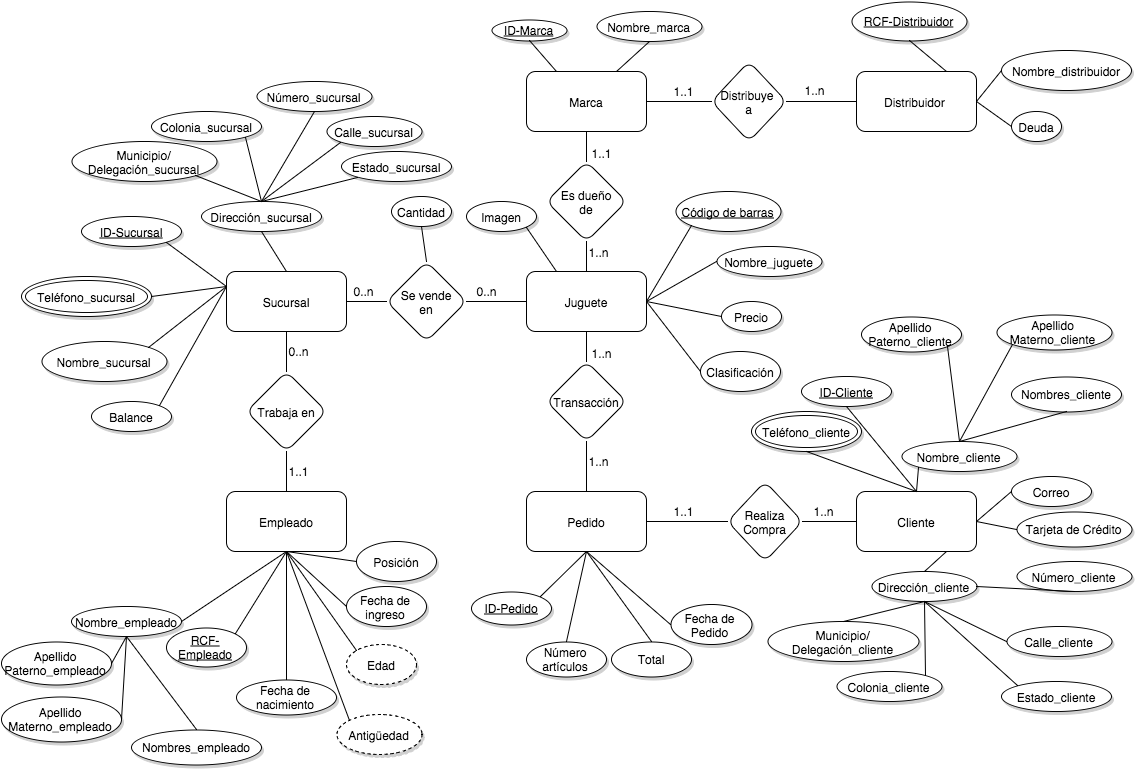
\includegraphics[width=10cm, height=10cm]{Pactica2} }
   
 \end{document}
